\newcommand{\svcourse}{CST Part IA: Software Engineering and Security}
\newcommand{\svnumber}{1}
\newcommand{\svvenue}{Microsoft Teams}
\newcommand{\svdate}{2022-05-11}
\newcommand{\svtime}{15:00}
\newcommand{\svuploadkey}{CBd13xmL7PC1zqhNIoLdTiYUBnxZhzRAtJxv/ytRdM1r7qIfwMsxeVwM/pPcIo8l}

\newcommand{\svrname}{Dr Sam Ainsworth}
\newcommand{\jkfside}{oneside}
\newcommand{\jkfhanded}{yes}

\newcommand{\studentname}{Harry Langford}
\newcommand{\studentemail}{hjel2@cam.ac.uk}


\documentclass[10pt,\jkfside,a4paper]{article}

\usepackage{stmaryrd}
\usepackage{tikz}
\usetikzlibrary{positioning, calc}

% DO NOT add \usepackage commands here.  Place any custom commands
% into your SV work files.  Anything in the template directory is
% likely to be overwritten!

\usepackage{fancyhdr}

\usepackage{lastpage}       % ``n of m'' page numbering
\usepackage{lscape}         % Makes landscape easier

\usepackage{verbatim}       % Verbatim blocks
\usepackage{listings}       % Source code listings
\usepackage{graphicx}
\usepackage{float}
\usepackage{epsfig}         % Embed encapsulated postscript
\usepackage{array}          % Array environment
\usepackage{qrcode}         % QR codes
\usepackage{enumitem}       % Required by Tom Johnson's exam question header

\usepackage{hhline}         % Horizontal lines in tables
\usepackage{siunitx}        % Correct spacing of units
\usepackage{amsmath}        % American Mathematical Society
\usepackage{amssymb}        % Maths symbols
\usepackage{amsthm}         % Theorems

\usepackage{ifthen}         % Conditional processing in tex

\usepackage[top=3cm,
            bottom=3cm,
            inner=2cm,
            outer=5cm]{geometry}

% PDF metadata + URL formatting
\usepackage[
            pdfauthor={\studentname},
            pdftitle={\svcourse, SV \svnumber},
            pdfsubject={},
            pdfkeywords={9d2547b00aba40b58fa0378774f72ee6},
            pdfproducer={},
            pdfcreator={},
            hidelinks]{hyperref}

\renewcommand{\headrulewidth}{0.4pt}
\renewcommand{\footrulewidth}{0.4pt}
\fancyheadoffset[LO,LE,RO,RE]{0pt}
\fancyfootoffset[LO,LE,RO,RE]{0pt}
\pagestyle{fancy}
\fancyhead{}
\fancyhead[LO,RE]{{\bfseries \studentname}\\\studentemail}
\fancyhead[RO,LE]{{\bfseries \svcourse, SV~\svnumber}\\\svdate\ \svtime, \svvenue}
\fancyfoot{}
\fancyfoot[LO,RE]{For: \svrname}
\fancyfoot[RO,LE]{\today\hspace{1cm}\thepage\ / \pageref{LastPage}}
\fancyfoot[C]{\qrcode[height=0.8cm]{\svuploadkey}}
\setlength{\headheight}{22.55pt}


\ifthenelse{\equal{\jkfside}{oneside}}{

 \ifthenelse{\equal{\jkfhanded}{left}}{
  % 1. Left-handed marker, one-sided printing or e-marking, use oneside and...
  \evensidemargin=\oddsidemargin
  \oddsidemargin=73pt
  \setlength{\marginparwidth}{111pt}
  \setlength{\marginparsep}{-\marginparsep}
  \addtolength{\marginparsep}{-\textwidth}
  \addtolength{\marginparsep}{-\marginparwidth}
 }{
  % 2. Right-handed marker, one-sided printing or e-marking, use oneside.
  \setlength{\marginparwidth}{111pt}
 }

}{
 % 3. Alternating margins, two-sided printing, use twoside.
}


\setlength{\parindent}{0em}
\addtolength{\parskip}{1ex}

% Exam question headings, labels and sensible layout (courtesy of Tom Johnson)
\setlist{parsep=\parskip, listparindent=\parindent}
\newcommand{\examhead}[3]{\section{#1 Paper #2 Question #3}}
\newenvironment{examquestion}[3]{
\examhead{#1}{#2}{#3}\setlist[enumerate, 1]{label=(\alph*)}\setlist[enumerate, 2]{label=(\roman*)}
\marginpar{\href{https://www.cl.cam.ac.uk/teaching/exams/pastpapers/y#1p#2q#3.pdf}{\qrcode{https://www.cl.cam.ac.uk/teaching/exams/pastpapers/y#1p#2q#3.pdf}}}
\marginpar{\footnotesize \href{https://www.cl.cam.ac.uk/teaching/exams/pastpapers/y#1p#2q#3.pdf}{https://www.cl.cam.ac.uk/\\teaching/exams/pastpapers/\\y#1p#2q#3.pdf}}
}{}


\begin{document}

\begin{examquestion}{2000}{6}{11}

\begin{enumerate}

\item For each of the given pairs of terms, give a most general unifier or
indicate why none exists. (Here $x$, $y$, $z$ are variables while $a$, $b$
are constant symbols.)

\begin{itemize}

\item $h(x, y, x)$ and $h(y, z, u)$
\[
\sigma = [x/y, x/z, x/u]
\]

\item $h(x, y, z)$ and $h(f(y), z, x)$

There is no most-general unifier. Unify the first parameter
using the most general unifier $\sigma=[f(y)/x]$. Leaving $h(f(y), y, z)$
and $h(f(y), z, f(y))$. Next unify the second parameter using the most
general unifier $\sigma = [y/z]$. This leaves $h(f(y), y, y)$ and $h(f(y),
y, f(y))$. Since $y$ and $f(y)$ cannot be unified, clearly the third
parameter cannot be unified.

\item $h(x, y, b)$ and $h(a, x, y)$

There is no most-general unifier. To unify the first parameters, we must use
the unifier $[x/a]$. This leaves the terms $h(a, y, b)$ and $h(a, a, y)$.
Now $y$ must be unified with both $a$ and $b$ -- this is not possible and
therefore there is no most general unifier.

\item $h(x, y, z)$ and $h(g(y, y), g(z, z), g(u, u))$
\[
\sigma =
[
g(g(g(u, u), g(u, u)), g(g(u, u), g(u, u)))/x, g(g(u, u), g(u, u))/y, g(u, u)/z
]
\]

\end{itemize}

A standard unification algorithm takes a pair of terms $t_1$ and $t_2$ and
returns a substitution $\theta$ such that $t_1\theta = t_2\theta$. Show how
this algorithm can be used to find the unifier of several $(n > 2)$ terms
$t_1, t_2, \dots, t_n$: a substitution $\theta$ such that $t_1\theta =
t_2\theta = \dots = t_n \theta$. Indicate how the unifier is constructed
from the unifiers of $n - 1$ pairs of terms. (Assume all required unifiers
exist and ignore the question of whether the unifiers are most general).

Its possible to apply unifiers to unifiers. For example, if the unifier
$\theta$ unifies $t_1$ and $t_2$; and the unifier $\phi$ unifies $t_1\theta$
and $t_3 \theta$; then $\psi = \theta \phi$ is a unifier for $t_1, t_2, t_3$
ie $t_1\psi = t_2\psi = t_3\psi $.

We can use this knowledge to define a unifier for all the terms inductively:
\begin{align*}
t_1\theta_1 &= t_2\theta_1 \\
t_1\theta_1 \theta_2 \dots \theta_i &= t_{i+1}\theta_1 \theta_2 \dots
\theta_i \\
\sigma &= \theta_1 \theta_2 \dots \theta_{n-1}
\end{align*}

With $A$ as the algorithm to find the most general unifier for two terms:
\begin{lstlisting}[language=python, mathescape=true]
terms = [$t_1$, $t_2$, ..., $t_n$]

$\sigma$ = []

for i in range(2, n + 1):
	$\theta$ = A($t_1$, terms[i])
	$\sigma$ = $\sigma\theta$
\end{lstlisting}

\item Prove using resolution the formula
\[
(\forall x[P(x)\leftrightarrow (Q(x) \wedge \neg Q(f(x)))]) \to \exists y
\neg P(y)
\]

The first stage is to negate the formula. Note this is an implication
$A \to B$ so the negation is of the form $A \wedge \neg B$. I will create
the clauses for $A$ and $B$ separately.
\begin{align*}
A =& \forall x[P(x)\leftrightarrow (Q(x) \wedge \neg Q(f(x)))] \\
=& \forall x. (P(x) \vee \neg (Q(x) \wedge \neg Q(f(x)))) \wedge
(\neg P(x) \vee (Q(x) \wedge \neg Q(f(x)))) \\
=& \forall x. (P(x) \vee \neg Q(x) \vee Q(f(x))) \wedge
(\neg P(x) \vee Q(x)) \vee (\neg P(x) \vee \neg Q(f(x))) \\
\intertext{Skolemizing gives:}
=& (P(x) \vee \neg Q(x) \vee Q(f(x))) \wedge
(\neg P(x) \vee Q(x)) \vee (\neg P(x) \vee \neg Q(f(x))) \\
=& \{P(x), \neg Q(x)\}\ \{\neg P(x), Q(x)\}\ \{\neg P(x), \neg Q(f(x))\} \\\\\\
B =& \neg \exists y \neg P(y) \\
=& \forall y \neg \neg P(y) \\
=& \forall y P(y) \\
\intertext{Skolemizing gives:}
=& P(y) \\
=& \{P(y)\} \\
\intertext{So the clauses for the whole expression are:}
& \{P(x), \neg Q(x)\}\ \{\neg P(x), Q(x)\}\ \{\neg P(x), \neg Q(f(x))\}\ \{P
(y)\} \\
\intertext{Variables are scoped only within their clause -- for clarity I
will rename to give unique names. Note this does not change the semantic
meaning.}
& \{P(w), \neg Q(w)\}\ \{\neg P(x), Q(x)\}\ \{\neg P(y), \neg Q(f(y))\}\ \{P
(z)\} \\
\end{align*}

\begin{align*}
& \{P(w), \neg Q(w)\}\ \{\neg P(x), Q(x)\}\ \{\neg P(y), \neg Q(f(y))\}\ \{P
(z)\} \\
\intertext{Use the unifiers $\sigma_1=[x/z]$ and $\sigma_2=[y/z]$ to create
two new clauses}
=& \{P(w), \neg Q(w)\}\ \{\neg P(x), Q(x)\}\ \{\neg P(y), \neg Q(f(y))\}\ \{P
(z)\}\ \{P(x)\}\ \{P(y)\} \\
=& \{P(w), \neg Q(w)\}\ \{P(x)\}\ \{\neg P(x), Q(x)\}\ \{P(y)\}\ \{\neg P
(y), \neg Q(f(y))\}\ \{P(z)\}\ \\
\intertext{Use resolution to create two new clauses}
=& \{P(w), \neg Q(w)\}\ \{P(x)\}\ \{\neg P(x), Q(x)\}\ \{P(y)\}\ \{\neg P
(y), \neg Q(f(y))\}\ \{P(z)\}\ \{Q(u)\}\ \{\neg Q(f(v))\} \\
\intertext{Use the unifier $\sigma_3=[f(v)/u]$ to create a new clause}
=& \{P(w), \neg Q(w)\}\ \{P(x)\}\ \{\neg P(x), Q(x)\}\ \{P(y)\}\ \{\neg P
(y), \neg Q(f(y))\}\ \{P(z)\}\ \{Q(u)\}\ \{Q(f(v))\}\ \{\neg Q(f(v))\} \\
\intertext{Resolve to derive the empty clause $\boxempty$}
=& \{P(w), \neg Q(w)\}\ \{P(x)\}\ \{\neg P(x), Q(x)\}\ \{P(y)\}\ \{\neg P
(y), \neg Q(f(y))\}\ \{P(z)\}\ \{Q(u)\}\ \{Q(f(v))\}\ \{\neg Q(f(v))\}\
\boxempty
\end{align*}
Since the empty clause $\boxempty$ has been derived, the clauses
are inconsistent. Since the clauses were formed from the Skolemization of
the negation of the original formula, the original formula must be
valid

\textbf{How should we lay this out?} This feels verbose -- and would
becomes unreasonable in difficult questions. However, removal of clauses for
clarity (even when explicitly stated) looks erroneous.

\end{enumerate}

\end{examquestion}

\begin{examquestion}{2004}{6}{9}

For each of the following statements, briefly justify whether it is true or
false.

\begin{enumerate}

\item Given any propositional logic formula $\psi$ that is a tautology,
converting $\psi$ to CNF will result in $\mathbf{t}$.

This is false. If $\phi$ is converted to CNF then all clauses are
tautological -- of the form $P \vee \dots \vee \neg P$ for some proposition
$P$. If the formula is converted to CNF and all tautological clauses are
deleted \textit{then} the formula will be $\mathbf{t}$.

Consider for example the tautological formula below, in CNF:
\[
(P \vee Q \vee \neg P) \wedge (Q \vee R \vee \neg P \vee \neg Q)
\]

\item Executing the DPLL method on the clauses
\[
\{P, Q, \neg S\}\ \{\neg P, Q, \neg R\}\ \{P\}\ \{\neg Q, R \}\ \{S, \neg Q\}
\]
produces a result without needing any case split steps.

This is false.

The DPLL method is as follows:
\begin{itemize}

\item Delete all tautological clauses (clauses of the form $\{P, \dots, \neg P\}$)

\item Delete all Unit clauses (clauses of the form $\{P\}$) and propagate the
truth value of the propositional formula in the unit clause.

\item Propagate any pure literals -- these are literals which only occur
either negated or non-negated -- it's possible to satisfy all clauses
containing them without restricting any other formulae. So shoud be done.

\item If none of the above are present then perform a case split -- try
case $P \mapsto 0$, if you fail then try case $P\mapsto 1$.

\item Repeat

\end{itemize}

Applying this method to the clauses above requires a case split:
\begin{gather*}
\{P, Q, \neg S\}\ \{\neg P, Q, \neg R\}\ \{P\}\ \{\neg Q, R \}\ \{S, \neg
Q\} \\
\intertext{Unit $P$}
\{Q, \neg R\}\ \{\neg Q, R \}\ \{S, \neg Q\} \\
\intertext{Pure S}
\{Q, \neg R\}\ \{\neg Q, R \}\ \\
\intertext{Case split!}
\end{gather*}

\item The OBDD corresponding to the propositional logical formula
$(P \vee Q) \wedge \neg P$ does not have any decision nodes for the
propositional letter $P$.

The statement is false.

The OBDD for the propositional formula is given below:
\begin{center}
\begin{tikzpicture}
\node (P) {$P$};
\node (Q) [below right = of P] {$Q$};
\node (0) [below left = of Q] {$0$};
\node (1) [below right = of Q] {$1$};
\path (P) edge [dashed] (Q);
\path (P) edge (0);
\path (Q) edge [dashed] (0);
\path (Q) edge (1);
\end{tikzpicture}
\end{center}
Clearly there is a decision node for the propositional letter $P$.

\item Skolemizing the first order logic formula $\exists x(\phi(x))$ results
in a logically equivalent formula $\phi(a)$ (where $a$ is a fresh constant).

This is false. Skolemization does not preserve meaning -- it only preserves
consistency. Therefore Skolemizing the formula $\exists x(\phi(x))$ does not
preserve logical meaning.

\item The Herbrand Universe that is generated from the clauses $\{P(a)\}$,
$\{Q(x, b), \neg P(x)\}$ and $\{\neg Q(a, y)\}$ contains two elements.

This is true. The Herbrand Universe for these clauses is defined as follows:
\begin{align*}
H_0 &= \{a, b\} \\
H_{i+1} &= \{f_n(x_1, \dots x_n)| x_1, \dots x_n \in H_i\} \\
\mathcal{H} &= \bigcup_{i \in \mathbb{N}} H_i
\end{align*}
Note, however that there are no functions -- therefore the sets $H_1, \dots
H_n$ are empty. So the Herbrand Universe $\mathcal{H}$ contains only the two
elements $\{a, b\}$.

\item The two terms $f(x, y, z)$ and $f(g(y, y), g(z, z), g(a, a))$ can
be unified.

This is true! The most general unifier is:
\[
\sigma = [g(g(g(a, a), g(a, a)), g(g(a, a), g(a, a)))/x, g(g(a, a), g(a, a))/y, g(a, a)/z]
\]

\item It is not possible to remove the clauses $\{P(x)\}$ and
$\{\neg P(f(x))\}$ because the \textit{occurs check} prevents the literals
being unified.

This is false!

The domain of a variable is within its own clause -- so the $x$ in each
clause is a \textit{different} universally bound variable.

The clauses are logically equivalent to $\{P(x)\}$, $\{\neg P(f(y))\}$ --
which can be unified to $\boxempty$ using the unifier $\sigma = [f(y)/x]$.

\item The clause $\{P(x, x), P(x, a)\}$ can be factored to give the new
clause $\{P(x, a)\}$.

This is false. The most-general unifier for $\{P(x, x)\}$ and $\{P(x, a)\}$ is
$\sigma = [a/x]$. This unifies the terms to $\{P(a, a)\}$ and $\{P(a, a)\}$.
This clause can then be factored to form the new clause $\{P(a, a)\}$. This
is \textbf{note} equivalent to $\{P(x, a)\}$.

\item The empty clause can be derived from the clauses $\{P(x), P(a)\}$,
$\{P(x), \neg P(a)\}$, $\{\neg P(b), Q\}$ and $\{\neg P(c), \neg Q\}$.

This is true.

\begin{itemize}

\item The clauses $\{\neg P(b), Q\}$ and $\{\neg P(c), \neg Q\}$ can be
unified, creating the clause $\{\neg P(b), \neg P(c)\}$.

\item The clauses $\{P(x), P(a)\}$ and $\{P(x), \neg P(a)\}$ can be unified
forming the clause $\{P(x)\}$

\item The clauses $\{P(x)\}$ and $\{\neg P(b), \neg P(c)\}$ can be unified
with the unifier $[b/x]$ then resolved to form the new clause $\{\neg P(c)\}$

\item The clauses $\{P(x)\}$ and $\{\neg P(c)\}$ can be unified with the
unifier $[c/x]$ then resolved to form the empty clause $\boxempty$

\end{itemize}

\item Because in the modal logic S4 the equivalence $\boxempty \boxempty
\phi \simeq \boxempty \phi $ holds for every formula $\phi $, it follows
that $\diamond\diamond\phi \simeq \diamond\phi $

This is true. We can derive $\diamond\diamond\phi \simeq \diamond\phi $
using the equivalence $\diamond \phi \simeq \neg \boxempty \neg \phi $

\begin{align*}
\boxempty \boxempty \phi &\simeq \boxempty \phi \Longleftrightarrow \\
\boxempty \boxempty \neg \phi &\simeq \boxempty \neg \phi \Longleftrightarrow \\
\neg \boxempty \boxempty \neg\phi &\simeq \neg \boxempty \neg\phi
\Longleftrightarrow \\
\diamond \neg \boxempty \neg\phi &\simeq \diamond \neg\neg\phi
\Longleftrightarrow \\
\diamond \diamond \neg\neg\phi &\simeq \diamond \neg\neg\phi
\Longleftrightarrow \\
\diamond \diamond \phi &\simeq \diamond \phi \\
\end{align*}

\end{enumerate}

\end{examquestion}

\begin{examquestion}{1998}{5}{10}

\begin{enumerate}

\item Construct an ordered binary decision diagram (OBDD) for the formula
\[
\left[ \left( P \to Q \right) \wedge \left( \neg R \vee \neg Q \right)
\right] \to \neg R
\]
showing each step carefully. What does the OBDD tell us about whether the
formula is $(a)$ valid and $(b)$ satisfiable and $(c)$ inconsistent?

Note that although I show logically equivalent expressions separately, they
point to the same BDD\@. I do this for clarity.

Firstly, consider the expression $P \to Q$
\begin{center}
\begin{tikzpicture}
\node (P) {$P$};
\node (0) [below left = of P] {$0$};
\node (1) [below right = of P] {$1$};
\path [dashed] (P) edge (0);
\path (P) edge (1);
\end{tikzpicture}
\hspace{1cm}
\begin{tikzpicture}
\node (P) {$Q$};
\node (0) [below left = of P] {$0$};
\node (1) [below right = of P] {$1$};
\path [dashed] (P) edge (0);
\path (P) edge (1);
\end{tikzpicture}
\end{center}
We can merge these using the $\to$ rule:
\begin{align*}
IF(P, 1, 0) \to IF(Q, 1, 0)
&= IF(P, 1 \to IF(Q, 0, 1), 0 \to IF(Q, 0, 1)) \\
&= IF(P, IF(Q, 1, 0), 1)
\end{align*}
So $P \to Q$ is represented by the BDD below:
\begin{center}
\begin{tikzpicture}
\node (P) {$P$};
\node (Q) [below left = of P] {$Q$};
\node (0) [below left = of Q] {$0$};
\node (1) [below right = of Q] {$1$};
\path (P) edge (Q);
\path [dashed] (P) edge (1);
\path [dashed] (Q) edge (0);
\path (Q) edge (1);
\end{tikzpicture}
\end{center}
Next consider the expression $\neg R \vee \neg Q$. Starting with $\neg R$
and $\neg Q$:
\begin{center}
\begin{tikzpicture}
\node (P) {$Q$};
\node (0) [below left = of P] {$1$};
\node (1) [below right = of P] {$0$};
\path [dashed] (P) edge (0);
\path (P) edge (1);
\end{tikzpicture}
\hspace{1cm}
\begin{tikzpicture}
\node (P) {$Q$};
\node (0) [below left = of P] {$1$};
\node (1) [below right = of P] {$0$};
\path [dashed] (P) edge (0);
\path (P) edge (1);
\end{tikzpicture}
\end{center}
We can merge these together using the $\vee$ rule:
\begin{align*}
IF(Q, 0, 1) \vee IF(R, 0, 1)
&= IF(Q, 0 \vee IF(R, 0, 1), 1 \vee IF(R, 0, 1)) \\
&= IF(Q, IF(R, 0, 1), 1) \\
\end{align*}
So the expression $\neg R \vee \neg Q$ forms the OBDD:
\begin{center}
\begin{tikzpicture}
\node (Q) {$Q$};
\node (R) [below left = of Q] {$R$};
\node (0) [below left = of R] {$0$};
\node (1) [below right = of R] {$1$};
\path [dashed] (Q) edge (1);
\path [dashed] (R) edge (1);
\path (Q) edge (R);
\path (0) edge (R);
\end{tikzpicture}
\end{center}
Next, merge these two expressions using the $\wedge$ rule:
\begin{align*}
 & IF(P, IF(Q, 1, 0), 1) \wedge IF(Q, IF(R, 0, 1), 1) \\
=& IF(P, IF(Q, 1, 0) \wedge IF(Q, IF(R, 0, 1), 1), 1 \wedge IF(Q, IF(R, 0,
1), 1)) \\
=& IF(P, IF(Q, 1 \wedge IF(R, 0, 1), 0 \wedge 1), IF(Q, IF(R, 0, 1), 1)) \\
=& IF(P, IF(Q, IF(R, 0, 1), 0), IF(Q, IF(R, 0, 1), 1))
\end{align*}
So the LHS of the implication forms the OBDD:
\begin{center}
\begin{tikzpicture}
\node (P) {$P$};
\node (Q1) [below right = of P] {$Q$};
\node (Q2) [below left = of P] {$Q$};
\node (R) [below left = of Q1] {$R$};
\node (0) [below left = of R] {$0$};
\node (1) [below right = of R] {$1$};
\path [dashed] (P) edge (Q1);
\path (P) edge (Q2);
\path (Q1) edge (R);
\path (Q2) edge (R);
\path [dashed] (Q2) edge (0);
\path [dashed] (Q1) edge (1);
\path (R) edge (0);
\path [dashed] (R) edge (1);
\end{tikzpicture}
\end{center}
We must now merge it with the RHS of the implication $\neg R$. This can be
done using the $\to$ rule.
\begin{align*}
 & IF(P, IF(Q, IF(R, 0, 1), 0), IF(Q, IF(R, 0, 1), 1)) \to IF(R, 0, 1) \\
=& IF(P, IF(Q, IF(R, 0, 1), 0) \to IF(R, 0, 1), IF(Q, IF(R, 0, 1), 1) \to IF(R, 0, 1)) \\
=& IF(P, IF(Q, IF(R, 0, 1) \to IF(R, 0, 1), 0 \to IF(R, 0, 1)),
IF(Q, IF(R, 0, 1) \to IF(R, 0, 1), 1 \to IF(R, 0, 1))) \\
=& IF(P, IF(Q, IF(R, 0 \to 0, 1 \to 1), 1), IF(Q, IF(R, 0 \to 0, 1 \to 1),
IF(R, 0, 1))) \\
=& IF(P, IF(Q, IF(R, 1, 1), 1), IF(Q, IF(R, 1, 1), IF(R, 0, 1)))
& \intertext{Note that the tests $IF(R, 1, 1)$ are redundant and can be
replaced by 1}
=& IF(P, IF(Q, 1, 1), IF(Q, 1, IF(R, 0, 1)))
& \intertext{The test $IF(Q, 1, 1)$ is redundant and can be replaced by 1}
=& IF(P, 1, IF(Q, 1, IF(R, 0, 1)))
\end{align*}
This is equivalent to the following BDD:
\begin{center}
\begin{tikzpicture}
\node (P) {$P$};
\node (Q) [below left = of P] {$Q$};
\node (R) [below = of Q] {$R$};
\node (0) [below = of R] {$0$};
\node (1) [below right = of R] {$1$};
\path [dashed] (P) edge (Q);
\path [dashed] (Q) edge (R);
\path [dashed] (R) edge (1);
\path (P) edge (1);
\path (Q) edge (1);
\path (R) edge (0);
\end{tikzpicture}
\end{center}

\end{enumerate}

\end{examquestion}

\end{document}
